\documentclass[11pt,acmsmall,nonacm]{acmart}

\settopmatter{printacmref=false}
\renewcommand\footnotetextcopyrightpermission[1]{}

\usepackage[utf8]{inputenc}
\usepackage[T1]{fontenc}
\usepackage{amsmath}
\usepackage{graphicx}
\usepackage{booktabs}
\usepackage{hyperref}
\usepackage[inline]{enumitem}
\usepackage{subcaption}
\usepackage{adjustbox}
\usepackage{lineno}
\linenumbers


% NOTES CMDS
\usepackage{ulem}
\newcommand{\LH}[1]{\textcolor{blue}{{ #1}}}
\newcommand{\LHs}[1]{\textcolor{blue}{\sout {#1}}}
\newcommand{\MH}[1]{\textcolor{red}{{ #1}}}
\newcommand{\MHs}[1]{\textcolor{red}{\sout {#1}}}
% END NOTES CMDS

\title{Exploring Graph Topologies in Quantum Annealing}
%\title{The Role of Topology in Quantum Annealing}
%\title{Mind the Graph: The Role of Topology in Quantum Annealing}

\author{Mario Bifulco}
\affiliation{%
  \institution{University of Turin}
  \city{Turin}
  \country{Italy}}
\email{mario.bifulco@unito.it}

\author{Luca Roversi}
\affiliation{%
  \institution{University of Turin}
  \city{Turin}
  \country{Italy}}
\email{luca.roversi@unito.it}

\begin{document}

\begin{abstract}
Quantum Annealing (QA) offers a promising framework for solving NP-hard optimization problems, but its effectiveness is constrained by the topology of the underlying quantum hardware. Solving an optimization problem $P$ via QA involves a hardware-aware compilation which requires representing $P$ as a graph $G_P$ and relating it to a minor of $G_Q$, with $G_Q$ being the hardware graph that defines how qubits connect to each other in a QA-based quantum processing unit (QPU).

Minor Embedding (ME) is a possible operational form of the hardware-aware compilation we are dealing with. ME heuristically builds a map that associates each node of $G_P$ --- the logical variables of $P$ --- to a chain of adjacent nodes in $G_Q$ by means of one of its minors, so that the arcs of $G_P$ are preserved as physical connections among qubits in $G_Q$.

The static topology of hardwired qubits can clearly lead to inefficient compilations because $G_Q$ cannot be a clique, currently. We propose a methodology and a set of criteria to evaluate how the hardware topology $G_Q$ can negatively affect the embedded problem, thus making the quantum optimization more sensible to noise.

We evaluate the result of ME across two QPU topologies: Zephyr graphs (used in current D-Wave systems) and Havel-Hakimi graphs, which allow controlled variation of the average node degree. This enables us to study how the ratio `number of nodes/number of incident arcs per node' affects ME success rates to map $G_P$ into a minor of $G_Q$.

Our findings, obtained through ME executed on classical, i.e. non-quantum, architectures, suggest that Havel–Hakimi–based topologies, on average, require shorter qubit chains in the minor  of $G_P$, exhibiting smoother scaling of the largest embeddable $G_P$ as the QPU size increases. These characteristics indicate their potential as alternative designs for QA-based QPUs.
\end{abstract}


\maketitle

\section{Introduction}

\subsection{Quantum annealing in the landscape of quantum computing}

In the current landscape of quantum computing, two principal paradigms can be identified.
The first is \emph{digital quantum computing}, which relies on quantum gates—the quantum counterpart of classical logic gates—and offers universality at the cost of high control and error-correction overhead.
The second is \emph{analog quantum computing}, typically realized through \emph{Adiabatic Quantum Computing} (AQC)~\cite{AQC}.
Although AQC is theoretically universal, no large-scale universal implementation has yet been demonstrated.
A practically relevant subset of AQC is \emph{Quantum Annealing} (QA)~\cite{QA}, a non-universal but effective approach for solving NP-hard optimization problems by exploiting quantum tunneling to explore complex energy landscapes.

\subsection{Workflow and compilation challenges}

The QA workflow can be schematically divided into three main stages:
\begin{enumerate*}
  \item Express the optimization problem $P$ in \emph{Quadratic Unconstrained Binary Optimization} (QUBO) form~\cite{lucas}, which entails representing $P$ as a weighted graph $G_P$, often a clique;
  \item Embed $G_P$ into the hardware graph $G_Q$ that encodes the physical topology of the quantum processing unit (QPU)~\cite{ME, MEdwave, MENP, localembedding};
  \item Execute the annealing process, during which the physical system described by $G_Q$ evolves toward a low-energy state encoding the solution of $P$.
\end{enumerate*}

The second stage of the compilation flow, known as minor embedding (ME), is a heuristic procedure that adapts the logical connectivity of the problem graph $P$ to the limited, non-clique topology $G_Q$ of current QPUs.
Since the structure of $G_Q$ constrains which problems can be efficiently embedded, the quality of this stage plays a key role in determining the performance of the overall computation.
For this reason, we aim to develop tools to assess and improve ME quality.


\paragraph{Minor embedding}
For completeness, recall that a graph $G_m$ is a \emph{minor} of another graph $G$ if it can be obtained from $G$ through a finite sequence of edge contractions and vertex or edge deletions.
A classical result in graph theory—the \emph{Robertson–Seymour theorem}—states that the set of all minors of a given graph is \emph{downward-closed} under the minor relation, and that any such family can be characterized by a finite number of \emph{forbidden minors}.

In QA, however, the objective is more concrete: given a problem graph $G_P$ and a hardware graph $G_Q$, the goal is to find a minor $G_m$ of $G_Q$ that is isomorphic to $G_P$.
In practical terms, this means associating each logical variable of $P$ (a node of $G_P$) with a chain of physically adjacent qubits (nodes of $G_Q$), while preserving the adjacency relations that encode the problem’s constraints.
An illustrative example is reported in Figure~\ref{fig:embedding}, where a triangular problem graph is embedded into a square-lattice hardware graph.

The main difficulty of this process lies in the fact that current QPUs cannot realize fully connected topologies.
Consequently, long chains of qubits are often required to emulate logical connections, increasing susceptibility to noise and reducing the effective precision of the quantum annealing step.

%We remark that the study of minor embedding has implications beyond quantum computing itself, as it shares structural analogies with placement and routing problems in VLSI design, where logical circuits must also be efficiently mapped onto physically constrained architectures.

\begin{figure}
  \centering
  \adjustbox{scale=0.65,center}{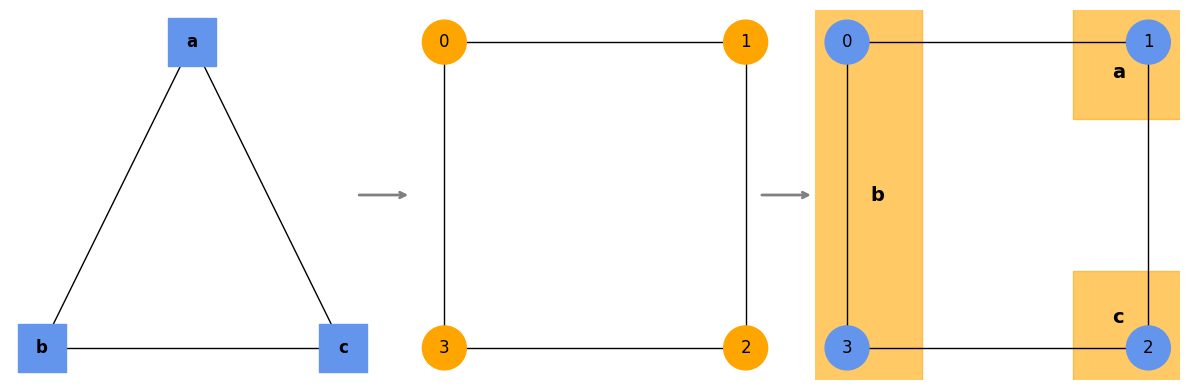
\includegraphics[width=\textwidth]{imgs/embedding.png}}
  \caption{Example of minor embedding: a problem graph $G_P$ (triangle) mapped onto the QPU topology $G_Q$ (square lattice), resulting in an embedded graph $G_E$.}
  \Description{Example of a problem graph $G_P$ with triangular connectivity embedded into a square-lattice QPU topology $G_Q$, forming the embedded graph $G_E$.}
  \label{fig:embedding}
\end{figure}

\subsection{Topological limitations and motivation for this study}

Recent generations of D-Wave annealers illustrate this trade-off between connectivity and scalability.
The Pegasus topology~\cite{Pegasus}, for instance, allows embeddings of up to roughly 100-variable cliques on a QPU with more than 5000 qubits~\cite{mscthesis}.
The more recent Zephyr topology, while featuring fewer physical qubits (around 4000), provides denser connectivity and can embed cliques up to approximately 150-varaible cliques.
Such differences highlight the crucial role of topology in determining the \LH{expressive power of a quantum annealer}, \LH{to us, ``expressive power'', in this context, meaning ``the average maximal dimension of a clique that can be minor embedded into an annealer.''}
This observation motivates a systematic study of how different QA-based QPUs topologies influence the embedded problem $G_E$.

\section{QPU Topology}

\LHs{The topology of a QPU, represented by its graph $G_Q$, determines the set of feasible embeddings and ultimately constrains the expressivity of quantum annealing.} \LH{(Trovo la frase una ripetizione du quanto detto poco prima)}
The topology can be analyzed at both coarse and fine granularity.
At a coarse level, metrics such as the number of nodes, edges, and the resulting average degree provide a global characterization \LH{, by which we mean $\ldots$}.
\LHs{However, embedding performance} \LH{(Non va bene cambiare termini. Con ``embedding performance'' intendiamo ancora ``expressive power'', secondo la definizione che ho provato ad abbozzare prima? Inltre, qui non è più necessario dire quanto già illustrato riguardo alla performance. Stai dicendo cosa è coarse e cosa è finer granularity.)} \LHs{depends strongly on the fine structure of $G_Q$:} \LH{At a finer level, it is known (\textbf{è noto?}) that metrics like} \emph{regularity}\LH{, i.e. (spiegazione?)\ldots}, \emph{modularity}\LH{, i.e. \ldots}, and \emph{degree distribution}, \LH{i.e. \ldots}, \LH{allow to highlight \ldots (elencare cosa evidenziano?) } \LHs{significantly affect how a problem graph $G_P$ can be mapped to form the embedded graph $G_E$}.

\LH{We are going to use the fine granularity metrics to compare Zephyr and Havel–Hakimi graph topologies of which Figure~\ref{fig:zephyr_hh} gives a pictorial comparison, relative to graphs of similar size and average degree.}

\begin{figure}
  \centering
  \begin{subfigure}{0.48\textwidth}
    \centering
    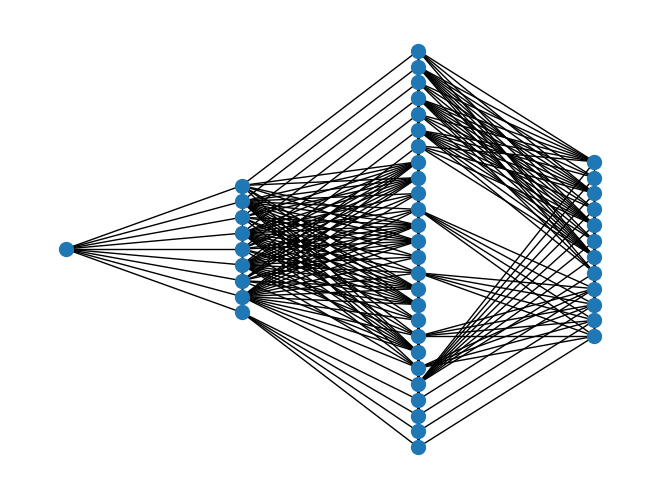
\includegraphics[width=\linewidth]{imgs/zephyr_bfs.png}
    \caption{Zephyr QPU topology $G_Q$ with parameters $m=1$, $t=4$.}
    \Description{Example of Zephyr QPU topology $G_Q$: parameters $m=1, t=4$.}
    \label{fig:zephyr_qpu}
  \end{subfigure}\hfill
  \begin{subfigure}{0.48\textwidth}
    \centering
    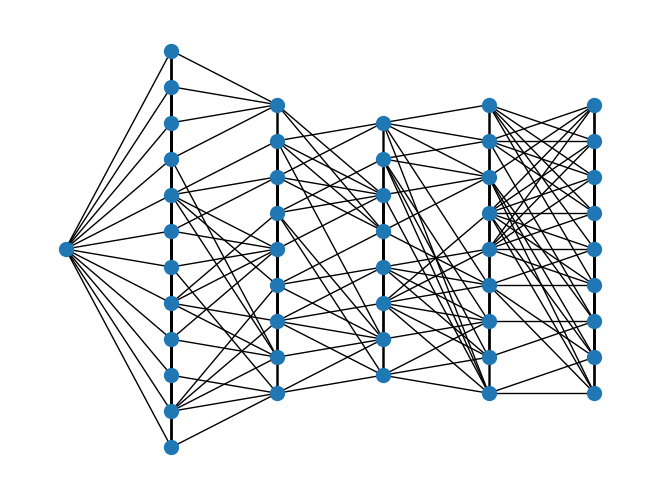
\includegraphics[width=\linewidth]{imgs/havel_hakimi.png}
    \caption{Havel-Hakimi QPU topology $G_Q$: 48 nodes of degree 12.}
    \Description{Example Havel-Hakimi QPU topology $G_Q$ with 48 nodes each one with degree 12.}
    \label{fig:hh_qpu}
  \end{subfigure}
  \caption{QPUs with comparable size and average degree but distinct structural properties.}
  \label{fig:zephyr_hh}
\end{figure}

\subsection{Zephyr Graph}
\LH{(Secondo me questa sezione è piuttosto inaccessibile. Credo serva una figura per far capire cos'è la \emph{grid} e cosa una \emph{tile}. Forse si può togliere l'attuale Fig 1. In fondo, è probabile che abbamo spiegato ragionevolmente bene cos'è ME.)}
The Zephyr graph~\cite{QPU} defines the current D-Wave QPU topology.
It is parameterized by the grid size $m$ and the tile size $t$, forming an $m \times m$ array of cross-shaped blocks, each with $t$ nodes extending from a central hub.
We explored configurations with $(m,t) \in [2,7] \times [1,25]$, generating 150 QPU graphs ranging from 40 to 10,500 nodes and 114 to 508,750 edges.

\subsection{Havel-Hakimi Graph}

Havel–Hakimi graphs are constructed by specifying the uniform node degree $deg$ and the total number of nodes $num\_qubits$.
The Havel–Hakimi algorithm~\cite{hh} iteratively connects nodes following a descending degree sequence, producing graphs with controlled degree distributions but limited structural regularity.
We generated regular instances with $deg \in \{5+25k \mid k=0,\dots,4\}$ and $num\_qubits \in \{50+350m \mid m=0,\dots,29\}$, yielding 150 graphs from 50 to 10,200 nodes and 125 to 535,500 edges. \LH{(Immagino che i parametri siano stati scelti per avere grafi con macro misure (numero nodi e archi) comparabili e poter procedere al loro confronto usando le metriche finemente granulari. Questo va detto esplicitamente, forse integrando il tutto quello che dici nel paragrafo ``Connectivity constraints.'' qui sotto. Tra l'altro ``Connectivity constraints'' è terminologia standard?)}

\paragraph{Connectivity constraints.}
Across all configurations, the maximum node degree was limited to approximately 100 to remain physically plausible.
Current architectures, such as Zephyr, achieve degrees up to 20; values beyond 100 \LH{would exceed foreseeable fabrication limits} \LH{(Quale fonte per la precedente affermazione?)}.
This constraint ensures that our exploration remains both physically grounded and indicative of future QPU scalability trends.

\section{Methodology}

We generated Zephyr and Havel–Hakimi graphs, \LH{standing for $G_Q$s,} using \texttt{zephyr\_graph} from \texttt{dwave\_networkx} and \texttt{havel\_hakimi\_graph} from \texttt{networkx}.
For each $G_Q$, we determined the largest embeddable clique $G_P = K_n$ using the \texttt{find\_embedding} function from \texttt{minorminer}.
The resulting embedded graph $G_E$ associates each node of $G_P$ with a chain of adjacent qubits in $G_Q$, preserving the logical adjacency structure.

\LH{We use \LH{$K_n$} cliques as benchmark because real-world QUBO instances $G_P$ often are highly connected graphs.}
%%%%%%%%%%%%%%%% Originale
%For each embedding, we collected:
%\begin{itemize}
%  \item Graph descriptors: type, parameters, number of nodes and edges, average degree;
%  \item Size of the largest embeddable clique;
%  \item Descriptive statistics (mean, median, mode) of qubit-chain lengths in $G_E$.
%\end{itemize}
\LH{(La versione originale di quel che segue l'ho commentata perché, se pensata, più o meno, in termini di formula logica, non mi pareva filasse.)}
Fixed $G_Q$, for each embedding of $K_n$ generating $G_E^{K_n}$, we collect:
\begin{itemize}
  \item the \emph{graph descriptors}: \emph{type}, \emph{parameters}, \emph{number of nodes} and \emph{edges}, \emph{average degree} $\tilde{\delta}_n$ \LH{of $K_n$?}, \LH{of $G_E^{K_n}$?};
  \item the \emph{descriptive statistics}: \emph{mean}, \emph{median}, and \emph{mode} of qubit-chain lengths in $G_E^{K_n}$.
\end{itemize}
Moreover, relatively to every $G_Q$, we record the size $\operatorname{\textit{max}}$ of the largest $K_{\operatorname{\textit{max}}} $ that ME can embed into $G_Q$, generating $G_E^{K_{\operatorname{\textit{max}}}}$.

Finally, for every $G_Q$, we normalize \LH{every} average degree $\tilde{\delta}_n$, and \LHs{the largest embeddable clique size} the value $\operatorname{\textit{max}}$ by the number of qubits in $G_Q$.
The normalization provides a unified comparison space to highlight structural correlations between QPU topologies and embedding performance \LH{because \ldots (secondo me una motivazione andrebbe data)}.

\section{Results}

\begin{figure}
  \centering
  \begin{subfigure}{0.48\textwidth}
    \centering
    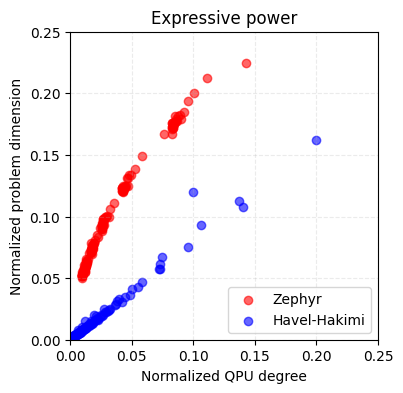
\includegraphics[width=\linewidth]{imgs/vs.png}
    \caption{Normalized size of embedded cliques $G_P$ across Zephyr and Havel–Hakimi QPU $G_Q$.}
    \Description{Scatter plot comparing the normalized clique size embeddable on Zephyr and Havel–Hakimi QPU graphs $G_Q$.}
    \label{fig:zephyr_vs_hh}
  \end{subfigure}\hfill
  \begin{subfigure}{0.48\textwidth}
    \centering
    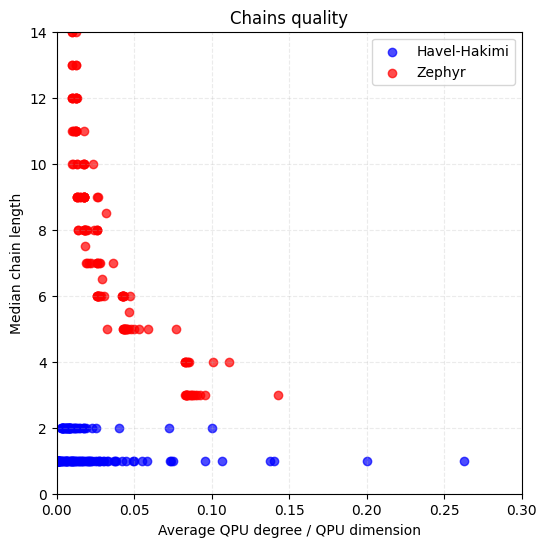
\includegraphics[width=\linewidth]{imgs/chains.png}
    \caption{\LHs{Median chain length in $G_E$ for each QPU configuration $G_Q$.} \LH{Median chain length among $G_E^{K_1} \ldots G_E^{K_{G_Q}}$ for every $G_Q$? Cambierei anche le didascalie nelle figure}}
    \Description{Median lengths of qubit chains in $G_E$ when $G_Q$ is Zephyr and Havel–Hakimi topology.}
    \label{fig:chains}
  \end{subfigure}
  \caption{Comparing \ldots \LH{(Senza questa caption non compare al numerazione per la figura 3.)}}
  \Description{Comparing \ldots}
  \label{fig:zephyr_vs_hh and chains}
\end{figure}

Figure~\ref{fig:zephyr_vs_hh} summarizes the results regarding the maximum size clique embeddable in a given QPU.
The horizontal axis represents the normalized average degree of $G_Q$, while the vertical axis reports the normalized size of the largest clique $G_P$ successfully embedded.
\LHs{Distinct scaling behaviors emerge for the two topologies.}

Havel–Hakimi graphs (blue points) display an almost linear scaling: as connectivity increases, the size of the embeddable clique grows proportionally.
Zephyr topologies (red points) exhibit a sublinear trend—highly expressive at low degrees but saturating as connectivity increases.

Figure~\ref{fig:chains} shows that embeddings on Havel–Hakimi graphs yield shorter qubit chains and smoother scaling.
Overall, these results suggest that synthetic topologies with controlled degree distributions can enhance embedding capacity without excessive chain length, thus improving robustness and scalability \LH{of solving problems by QA(?)}.

\section{Future work}

Future work will extend this comparative analysis to a broader set of synthetic and physically inspired QPU topologies $G_Q$.
We also plan to investigate correlations between structural indicators of $G_Q$ and practical embedding quality metrics, such as chain stability and noise susceptibility in $G_E$.
As a further direction, we intend to explore new candidate topologies derived from graph-theoretical principles, focusing on structures that could minimize the length of qubit chains while maintaining feasible connectivity and manufacturability.
These studies aim to support the co-design of hardware architectures and embedding heuristics, promoting QPU topologies that balance physical realizability, connectivity, and embedding efficiency.

\bibliographystyle{ACM-Reference-Format}
\bibliography{ref}

\end{document}
